\documentclass[12pt,letterpaper]{standalone}
\usepackage{pgf, tikz}
\usetikzlibrary{arrows, automata}
\usepackage{mwe} % For dummy images 
\usetikzlibrary{positioning}


\begin{document}
	
	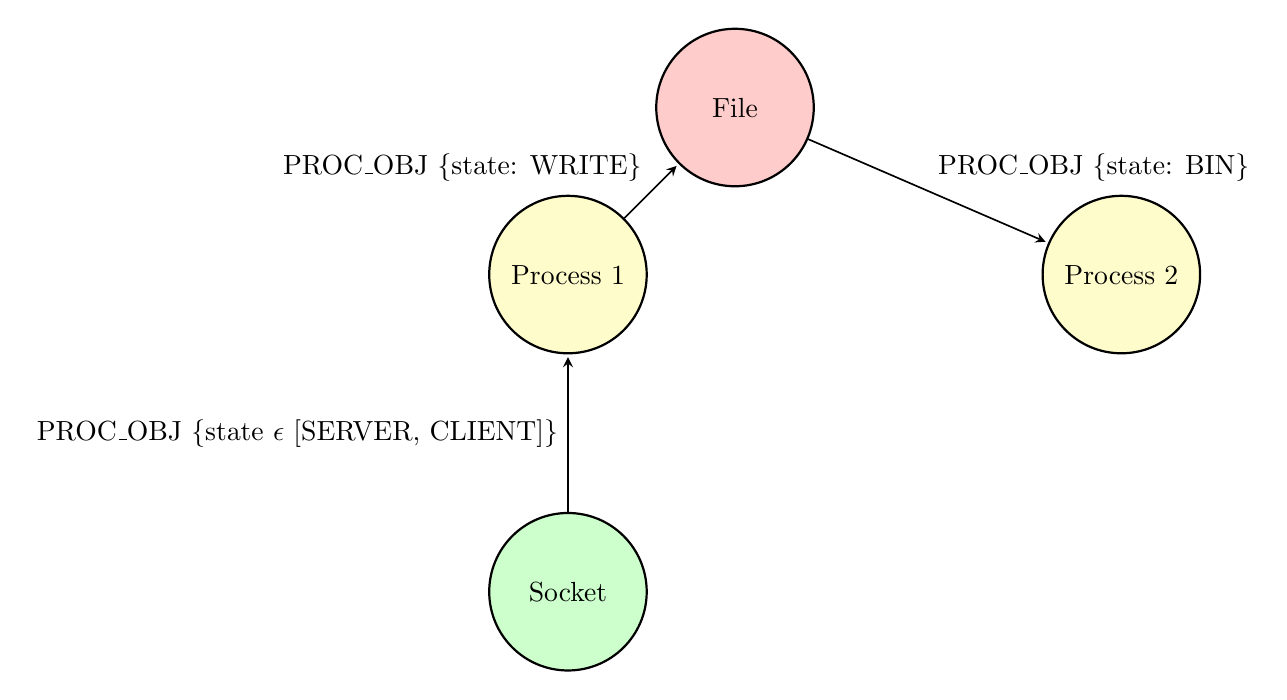
\begin{tikzpicture}[
	> = stealth, % arrow head style
	shorten > = 1pt, % don't touch arrow head to node
	auto,
	node distance = 3cm, % distance between nodes
	semithick % line style
	]
	
	\tikzstyle{every state}=[
	draw = black,
	thick,
	fill = white,
	minimum size = 20mm
	]
	
	\node[state, fill=yellow!20] (s) {Process 1};
	\node[state, fill=red!20] (v1) [above right of=s] {File};
	%\node[state] (v2) [right of=s] {$v_2$};
	\node[state, fill=green!20] (v3) [below=2cm of s] {Socket};
	\node[state, fill=yellow!20] (t) [right=5cm of s] {Process 2};
	
	\path[->] (s) edge node {PROC\_OBJ \{state: WRITE\}} (v1);
	%\path[->] (s) edge node {1} (v2);
	\path[->] (v3) edge node {PROC\_OBJ \{state $\epsilon$ [SERVER, CLIENT]\} } (s);

	%\path[->] (v3) edge node {1} (v2);
	\path[->] (v1) edge node {PROC\_OBJ \{state: BIN\}} (t);
	
	\end{tikzpicture}
	
\end{document}